\documentclass[11pt]{ctexart}

\usepackage{geometry}
\geometry{
    left = 0.6in,
    right = 0.6in,
    top = 0.8in,
    bottom = 1.0in
}
\usepackage{amssymb,amsbsy,amsmath,xcolor,mathrsfs,graphicx}
\usepackage{listings}
\usepackage{tasks}
\settasks{
    label = \Alph*. ,
    label-width = 16pt
}

\renewcommand{\title}[3]{
    \begin{center}
        \Large\heiti 中国电子学会 #1~年~#2~月 Python~#3级考试
    \end{center}
}
\newcommand{\TimeAndName}[1]{
    \begin{center}
        考试时间:~#1~ 分钟 \qquad\qquad\qquad\qquad 姓名:\underline{\quad\quad\quad\quad}
    \end{center}
}

\begin{document}
    \lstset{
        language = python,
        keywordstyle = \color{orange}\bfseries,
        emph = {
            abs, all, any, ascii, bin, bool, breakpoint, bytearray, bytes,
            callable, chr, classmethod, compile, complex, copyright, credits,
            delattr, dict, dir, divmod, enumerate, eval, exec, exit, filter,
            float, format, frozenset, getattr, globals, hasattr, hash,
            help, hex, id, input, int, isinstance, issubclass, iter, len,
            license, list, locals, map, max, memoryview, min, next, object,
            oct, open, ord, pow, print, property, quit, range, repr, reversed,
            round, set, setattr, slice, sorted, staticmethod, str, sum, super,
            tuple, type, vars, zip,
        },
        emphstyle = \color{purple}\bfseries,
        showspaces = false,
        basicstyle = \ttfamily,
        morekeywords = {True,False}
    }

    \title{2020}{9}{一}
    
    \TimeAndName{60}
    
    {\noindent\heiti 第一部分、单选题(共 25 题,每题 2 分,共50分.)}

    \begin{enumerate}
        % 1
        \item Python 自带的编程环境是?(\qquad)
        \begin{tasks}(4)
            \task PyScripter
            \task Spyder
            \task Notepad++
            \task IDLE
        \end{tasks}

        % 2
        \item 关于以下代码的说法正确的是?(\qquad)
        \begin{lstlisting}
            t = int(turtle.textinput("边数,几边形:"))
            turtle.circle(50, steps=t)
            turtle.done()
        \end{lstlisting}
        \begin{tasks}
            \task \lstinline{circle} 是画圆的代码,因此该程序运行后的图案一定是圆
            \task 运行该程序后,需要用户自己输入边数,确定画“几边形”
            \task 变量 \lstinline{t} 没有给出具体的数值,因此该程序运行有错误
            \task 改程序运行后,会画出 50 个圆
        \end{tasks}

        % 3
        \item Python 中幂运算符为?(\qquad)
        \begin{tasks}(4)
            \task \lstinline{*}
            \task \lstinline{*+}
            \task \lstinline{**}
            \task \lstinline{/}
        \end{tasks}

        % 4
        \item 下面代码的运行结果是?(\qquad)
        \begin{lstlisting}
            import turtle
            g = turtle.Pen()
            g.fillcolor("red")
            g.begin_fill()
            g.circle(50)
            g.pencolor("yellow")
            g.fillcolor("green")
            g.circle(50, steps=5)
            g.end_fill()
        \end{lstlisting}
        \begin{tasks}(4)
            \task 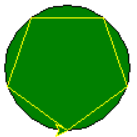
\includegraphics[width=.08\textwidth]{4a.png}
            \task 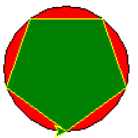
\includegraphics[width=.08\textwidth]{4b.png}
            \task 
\includegraphics[width=.08\textwidth]{4c.png}
            \task 
\includegraphics[width=.08\textwidth]{4d.png}
        \end{tasks}

        % 5
        \item 假设\lstinline{a = 20}, \lstinline{b = 3}, 那么 \lstinline{a or b} 的结果是?(\qquad)
        \begin{tasks}(4)
            \task $20$
            \task $0$
            \task $1$
            \task $3$
        \end{tasks}

        \newpage
        % 6
        \item 假设\lstinline{a = 2}, \lstinline{b = 3}, 那么\lstinline{a - b * b}的结果是?(\qquad)
        \begin{tasks}(4)
            \task $-3$
            \task $-2$
            \task $-7$
            \task $-11$
        \end{tasks}

        % 7
        \item 以下选项中不符合 Python 变量命名规则的是?(\qquad)
        \begin{tasks}(4)
            \task \lstinline{name}
            \task \lstinline{2_to}
            \task \lstinline{_Go}
            \task \lstinline{Tea}
        \end{tasks}

        % 8
        \item 创建一个新的 Python 程序,编写了下面的代码
        \begin{lstlisting}
            import turtle
            turtle.shape("turtle")
        \end{lstlisting}
        保存这个 Python 文件并且取了文件名.以下哪个文件名程序可以正常运行?(\qquad)
        \begin{tasks}(4)
            \task frist.py
            \task turtle.py
            \task import.py3
            \task hao.sb2
        \end{tasks}

        % 9
        \item 以下代码运行的结果是?(\qquad)
        \begin{lstlisting}
            a = "110"
            b = "9"
            c = a + b
            print(c)
        \end{lstlisting}
        \begin{tasks}(4)
            \task \lstinline{a + b}
            \task $119$
            \task \lstinline{c}
            \task $1109$
        \end{tasks}

        % 10
        \item IDLE 环境的退出命令是?(\qquad)
        \begin{tasks}(4)
            \task \lstinline{esc()}
            \task \lstinline{close()}
            \task 回车键
            \task exit()
        \end{tasks}

        % 11
        \item Python 中的整除运算符是用哪个符号表示的?(\qquad)
        \begin{tasks}(4)
            \task \lstinline{\\}
            \task \lstinline{//}
            \task \lstinline{\%}
            \task \lstinline{**}
        \end{tasks}

        % 12
        \item 执行语句 \lstinline{x, y = 9%5, 8//3} 后,变量 \lstinline{x}, \lstinline{y} 的之分别为?(\qquad)
        \begin{tasks}(4)
            \task \lstinline{18, 2}
            \task \lstinline{1, 2.66666}
            \task \lstinline{4, 2}
            \task \lstinline{1, 2}
        \end{tasks}

        % 13
        \item Python 注释方式正确的是?(\qquad)
        \begin{tasks}(2)
            \task \lstinline{//} 这是我的第一个程序
            \task \lstinline{\#} 程序的功能是输入Hello World
            \task \lstinline{?} 这个程序是用来计算两个数之和的
            \task \lstinline{**} 第一个Python程序 \lstinline{**}
        \end{tasks}

        \newpage
        % 14
        \item Python 中的 \verb|==| 代表的是?(\qquad)
        \begin{tasks}(2)
            \task 把左边的值赋值给右边
            \task 把右边的值赋值给左边
            \task 比较左右两边是否相等
            \task 左右两边值进行交换
        \end{tasks}
        
        % 15
        \item 以下代码哪部分是设置画布的颜色?(\qquad)
        \begin{lstlisting}
            import turtle
            turtle.screensize(_1_,_2_,_3_)
        \end{lstlisting}
        \begin{tasks}(4)
            \task 1
            \task 2
            \task 3
            \task 都不是
        \end{tasks}

        % 16
        \item 下面哪一行代码的输出结果不是 \lstinline{Python3.7} ?(\qquad)
        \begin{tasks}(2)
            \task \lstinline{print("Python3.7")}
            \task \lstinline{print("Python" + 3.7)}
            \task \lstinline{print("Python" + str(3.7))}
            \task \lstinline{print("Python" + "3.7")}
        \end{tasks}

        % 17
        \item 下列程序绘制的是一个什么图形?(\qquad)
        \begin{lstlisting}
            import turtle
            turtle.forward(100)
            turtle.left(120)
            turtle.forward(100)
            turtle.left(120)
            turtle.forward(100)
            turtle.left(120)
        \end{lstlisting}
        \begin{tasks}(4)
            \task 等边三角形
            \task 正方形
            \task 矩形
            \task 圆
        \end{tasks}

        % 18
        \item 使用下面中的哪个函数接收输入的数据?(\qquad)
        \begin{tasks}(4)
            \task accept()
            \task input()
            \task readline()
            \task login()
        \end{tasks}

        % 19
        \item \lstinline{turtle.color("red","yellow")} 命令中定义的颜色分别为?(\qquad)
        \begin{tasks}(2)
            \task 背景为黄色,画笔为红色
            \task 背景为红色,画笔为黄色
            \task 画笔为红色,填充为黄色
            \task 画笔为黄色,填充为红色
        \end{tasks}

        % 20
        \item \lstinline{print()} 的作用是什么?(\qquad)
        \begin{tasks}(2)
            \task 在屏幕上打印出来相应的文本或者数字等
            \task 在打印机里打印相关文本或者数字等
            \task 可以用来画图
            \task 输出一个命令行
        \end{tasks}

        % 21
        \item 下面的哪一个命令不是移动画笔箭头位置的命令?(\qquad)
        \begin{tasks}(4)
            \task \lstinline{turtle.forward()}
            \task \lstinline{turtle.goto()}
            \task \lstinline{turtle.color()}
            \task \lstinline{turtle.right()}
        \end{tasks}   

        % 22
        \item \lstinline{a = 2}, \lstinline{b = 3},那么\lstinline{c = a ** b} 运算的结果是?(\qquad)
        \begin{tasks}(4)
            \task 6
            \task 8
            \task 9
            \task 23
        \end{tasks}

        % 23
        \item 使用 Python 画笔绘制如下图所示的图案,第4行的代码应如何补充?(\qquad)
        
        \begin{minipage}{.46\textwidth}
            \centering
            \begin{lstlisting}
                import turtle
                p = turtle.Pen()
                p.forward(100)
                #4 _________
                p.forward(100)
                turtle.done()
            \end{lstlisting}
        \end{minipage}
        \begin{minipage}{.48\textwidth}
            \centering
            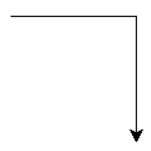
\includegraphics[width=.25\textwidth]{23.png}
        \end{minipage}

        \begin{tasks}(4)
            \task \lstinline{p.right(90)}
            \task \lstinline{p.left(90)}
            \task \lstinline{p.right(-90)}
            \task \lstinline{p.left(-90)}
        \end{tasks} 

        % 24
        \item 下面的运算符中,按照运算优先级哪一个是最高级
        \begin{tasks}(4)
            \task \lstinline{**}
            \task \lstinline{*}
            \task \lstinline{+}
            \task \lstinline{<}
        \end{tasks}

        % 25
        \item 下列数据中,不可能表示十六进制数的是?(\qquad)
        \begin{tasks}(4)
            \task \lstinline{ABC}
            \task \lstinline{17F}
            \task \lstinline{8H5}
            \task \lstinline{9a01}
        \end{tasks}
    \end{enumerate}

    {\noindent\heiti 第二部分、判断题(共 10 题,每题 2 分,共20分.)}
    \begin{enumerate}
        \setcounter{enumi}{25}
        % 26
        \item 以下三种表示字符串的方式都是正确的.(\qquad)
        \begin{lstlisting}
            "Hello"
            '不错'
            "我们一起走吧'
        \end{lstlisting}

        %27
        \item \lstinline{Turtle} 库是一个直观有趣的图形绘制函数库.(\qquad)
        
        %28
        \item 在 Python 中变量需要提前定义,可以不用赋值.(\qquad)
  
        %29
        \item 使用 \lstinline{Turtle} 时,画布默认坐标左上角为画布中心.(\qquad)
        
        %30
        \item \lstinline{print('hello,world')}和\lstinline{print('hello','world')}输出的内容一致
        
        %31
        \item Python 是交互式语言,这意味着,你可以在一个Python提示符 \lstinline!>>>! 后直接执行代码.(\qquad)
        
        %32
        \item \lstinline{print(int(8>7) or int(8<6))}的输出结果为1.(\qquad)
        
        %33
        \item import 可以作为变量名.(\qquad)
        
        %34
        \item 已知 \lstinline{y = 5}, 那么赋值语句 \lstinline{y = 'cedf'} 是无法正常执行的. (\qquad)
        
        %35
        \item Python2.x 编写的程序,在 Python3.x 都能正确打开并执行.(\qquad)
    \end{enumerate}

    {\noindent\heiti 第三部分、编程题(共 2 题,共30分.)}
    \begin{enumerate}
        \setcounter{enumi}{35}
        
        % 36
        \item 分解三位数:
        \begin{tasks}[label = (\arabic*)]
            \task 程序开始运行后,输入一个三位数整数;
            \task 程序会根据输入的整数输出百位、十位和个位上的数.例如,

            {\heiti 输入:}123

            {\heiti 输出:}百:1,十:2,个:3
        \end{tasks}
        \vfill

        %37
        \item 绘制图形:
        
        \begin{tasks}[label = (\arabic*)]
            \task 画一个边长为 200 的正方形,里面嵌套一个直径为 100 的圆,如下图;
            \task 圆的填充颜色为蓝色,所有的线条为黑色.
            \task 圆心位置为画布正中心.
        \end{tasks}
        \begin{center}
            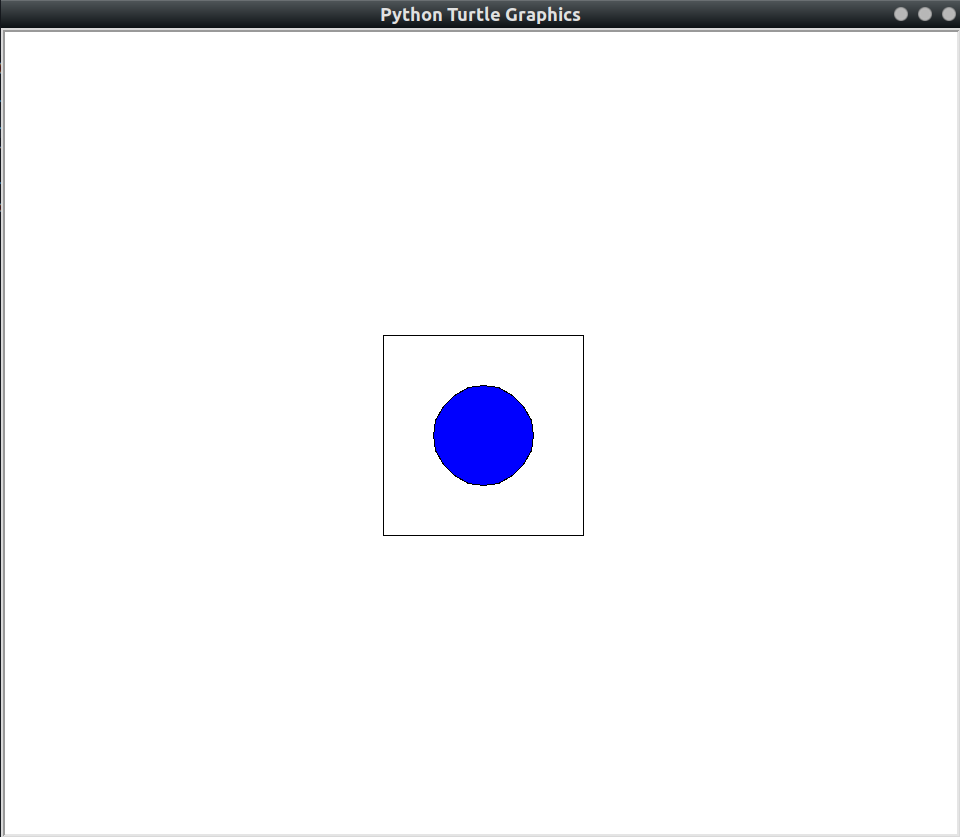
\includegraphics[width=.4\textwidth]{37.png}
        \end{center}
        \vfill
    \end{enumerate}
\end{document}